\graphicspath{{./communication/}}
\chapter{Arbeitspaket Kommunikation}
Für die Analyse, den Entwurf, die Impelementierung dieses Arbeitspaketes übernahm Herr Schleinkofer die Verantwortung. Während der Integration des Arbeitspaketes war Herr Schleinkofer unterstützend eingebunden.
\paragraph{}
Da die Projektspezifikation einen Datenaustausch zwischen $\mu$-Controller und PC enthält, muss diese auch im Projekt realisiert werden. Dabei kann sich auch am ISO/OSI-Schichtenmodell für Netzwerkkommunikation orientiert werden.
\section{Analysephase}
\subsection{Hardware}
Wie auch in der Physical-Layer behandelt, muss die Kommunikation in diesem Projekt zunächst physikalisch erfolgen. 
Dabei stellt sich die Frage, welche Möglichkeiten der Controller zur Datenübertragung an ein externes Gerät bietet. In dessen Handbuch ist aufgeführt, dass dort ein Universal Serial Interface Channel (USIC) Baustein zur Verfügung steht. Dies würde eine serielle Kommunikationsverbindung mit dem Universal Asynchronous Receiver Transmitter (UART) ermöglichen. Weitere Möglichkeiten sind auf dem Evaluation Board kaum gegeben. Dieses ist zwar für Ethernet vorbereitet, jedoch müssen dafür ein zusätzlicher Chip und eine RJ45-Buchse nachgerüstet werden. Eine selbst definierte und implementierte parallele Schnittstelle mit den GPIO-Ports wäre theoretisch auch möglich, jedoch in der Umsetzung zu komplex und zeitintensiv.
\paragraph{}
Die gemachten Überlegungen haben zur Folge, dass die Kommunikation zwischen Testplatz und PC über die serielle Schnittstelle abgewickelt wird. Nun muss entschieden werden, welches Gerät am Computer verwendet werden soll. Möglich wäre eine Kommunikation über ein serielles Kabel, welches an eine EIA-232 Schnittstelle des PC's angeschlossen wird. Dies ist jedoch mit einigen Problemen behaftet. Zunächst verfügen moderne Desktop Computer nur noch in wenigen Fällen über eine dedizierte EIA-232 Schnittstelle. Dies kann jedoch durch Verwendung eines USB-zu-Seriell-Adapters umgangen werden. Am $\mu$-Controller erfolgt dann der Anschluss an die GPIO-Pins. Allerdings muss dafür ein Adapter angefertigt werden, welcher auf der einen Seite einen D-Sub 9 Stecker und auf der anderen Seite mindestens die Pins 2 (Data Transceive), 3 (Data Receive) und 5 (Ground) als Stifte, passend zur Buchsenleiste des Evaulation Boards, weiterführt. Allerdings werden die Daten an der EIA-232 Schnittstelle mit bis zu 9 Volt übertragen. Dies stellt ein weiteres Problem dar, da an den Pins des Controllers nur 3,3 oder 5 Volt ausgegeben werden können. Auch kann ein Eingangssignal mit 9 Volt zu Schäden am $\mu$-Controller führen. Um dieses Problem zu umgehen, wäre es möglich, einen USB-zu-Seriell-Adapter mit integriertem Wandler-Chip zu verwenden.
\paragraph{}
Eine weitere Möglichkeit zur seriellen Kommunikation zeigt ein Beispielprojekt von Infineon für das Evaluation Board auf. In diesem erfolgt die Kommunikation zwischen PC und Controller über das USB-Kabel, welches am Debugging-Chip des Boards angeschlossen wird. Auch in diesem Projekt erfolgt der Datenaustausch mit Nutzung des USIC-Bausteins. Allerdings werden hier die Sende- und Empfangsleitungen an den XMC4200 Debug IC (im folgenden auch Debug-Chip genannt) auf der Platine weitergeleitet. Für den PC ist darüber hinaus ein Windows-Treiber verfügbar, welcher einen "virtuellen Com-Port" zur Kommunikation mit dem Evaluation Board einrichtet und über den nun Daten im Rahmen des Beispielprojektes ausgetauscht werden können. Auf die Software des PC's hat diese Vorgehensweise keinen Einfluss, da ein virtueller Com-Port in der gleichen Weise verwendet wird, wie ein Hardware-Gerät. Ein weiterer Vorteil dieser Lösung ist, dass eine zusätzliche Stromversorgung des $\mu$-Controllers entfällt, da dies über das USB-Kabel der Kommunikation erfolgt.
\paragraph{}
Die Aufgaben der zweiten Schicht des ISO/OSI-Modells umfassen unter Anderem auch die Sicherung der Datenintegrität während der Übertragung. Dies geschieht im Fall des Ethernet-Protokolls mittels eines Cyclic Redundancy Check Verfahrens. Und auch andere Kommunikationsprotokolle nutzen diese Art der Integritätsprüfung um etwaigen Störungen während der Übertragung entgegenzuwirken.
\paragraph{}
Weitere Funktionen aus höheren Schichten des ISO/OSI-Modells scheinen in der gegebenen Zeit nicht umsetzbar oder werden schlichtweg nicht benötigt. Eine Adressierung der Kommunikationspartner ist in diesem Fall aufgrund der auf genau zwei beschränkten Anzahl an Teilnehmern genausowenig notwendig wie eine Sitzungsverwaltung ähnlich derer in OSI-Schicht 5. Eine Flusskontrolle oder Empfangsbestätigung ist im Falle zu übertragender Sensordaten auch nicht sinnvoll. Diese Sensordaten sollen nach den Anforderungen regelmäßig vom $\mu$-Controller an den PC gesendet werden. Bei höheren Drehgeschwindigkeiten des Motors würden diese nur unnötig Rechenzeit auf der Senderseite verbrauchen. Bei der Übertragung von Regelungsparametern allerdings könnte eine Empfangsbestätigung durch den $\mu$-Controller durchaus nützlich sein. Allerdings ist hierzu wie bereits erwähnt der Zeitrahmen zu eng gesteckt.
\subsection{Software}
Des weiteren muss noch Analysiert werden, wie die Sensor- und Regelungsdaten für die Kommunikation aufbereitet werden. Hierzu kommen verschiedene Serialisierungsverfahren in Betracht. Zunächst besteht die Möglichkeit die Daten als String zu formatieren und die einzelnen Zeichen als char-Daten seriell zu übertragen. Dies ist eine einfache Lösung, jedoch für zukünftige Änderungen nur schlecht erweiterbar. Es muss dazu für jeden Sensor die komplette Decodierungs-Routine des Strings auf beiden Kommunikationspartnern angepasst werden. Sollten nun in Zukunft beispielsweise mehr Experimentierplätze mit unterschiedlichen Sensoren existieren, muss darauf geachtet werden, dass zu jedem auch ein PC verwendet wird, dessen GUI auch den String mit den vorliegenden Sensorwerten auswerten kann.
\paragraph{}
Alternativ dazu kann ein Serialisierungsformat mit dem Namen "Protocol Buffers" (kurz: Protobuf)  verwendet werden. Dieses wurde durch die Firma Google entwickelt und ist für mehrere Programmiersprachen verfügbar. Dies ist wichtig, da die Software auf dem $\mu$-Controller in C, der Teil für den PC aber in C\# geschrieben wird. Der Vorteil dieser Lösung besteht darin, dass etwaige neu hinzukommende Sensoren einfach in die Protobuf-Nachrichten aufgenommen werden können. Kann eine Gegenstelle diesen Teil einer Nachricht nicht verarbeiten, so wird dieser einfach ignoriert.
\paragraph{}
\begin{lstlisting}[caption=Beispieldefinition einer Protocol Buffers Nachricht, label=lst:protoEx]
message Person {
  required string name = 1;
  required int32 id = 2;
  optional string email = 3;
}
\end{lstlisting}
Dies liegt in der Art, wie eine Nachricht in Protobuf aufgebaut ist. Zunächst wird diese in einer Beschreibungssprache definiert.
Im Code \ref{lst:protoEx} ist ersichtlich, dass eine "Message" aus mehreren Feldern und deren zugehörigen Identifiern ("= 1" für das Feld "name") besteht. Wird nun eine Nachricht um neue Felder erweitert, so kann ein Programm, welches jedoch noch die alte Beschreibung nutzt, eine neuartige Nachricht wieder deserialisieren. Die neuen Felder jedoch werden hierbei aufgrund des unbekannten Identifiers ignoriert. Protobuf verfügt darüber hinaus noch über einen Codegenerator. Das bedeutet: Der Entwickler definiert in der gezeigten Beschreibungssprache eine Nachricht. Anhand dieser Beschreibung wird nun duch den Generator zum Beispiel C\#-Code zur De-/Serialisierung erstellt. Zusätzlich wird dabei eine Datenstruktur definiert, die vom Entwickler im Programmcode mit den zu übertragenden Daten ausgefüllt werden und einfach in einen Bytestream verwandelt und wieder zurückverwandelt werden kann.
\paragraph{}
Zwar gibt es keine "offizielle" Implementierung von Protobuf für C, jedoch existiert ein Projekt mit dem Namen "nanopb" welches die grundlegenden Funktionen von Protocol Buffers in C speziell für Embedded Systems umsetzt.
\section{Entwurfsphase}
Der Ablauf der Kommunikation sollte relativ einfach gehalten werden, um in der vorgegebenen Zeit umsetzbar zu sein. Daher senden die Kommunikationspartner nur einfache Protobuf-Nachrichten. Der PC sendet Regelungsparameter und Ziel an den Controller. Dieser wiederum sendet regelmäßig die Daten der angeschlossenen Sensoren an die GUI auf dem PC. Um die Kommunikation für die angrenzenden Arbeitspakete so einfach wie möglich zu gestalten, soll die Schnittstelle nur aus wenigen Funktionen bzw. Methoden bestehen.
\subsection{Nachrichtendefinition}
Im System gibt es zwei Arten von Nachrichten. Die erste Art enthält die gesammelten Daten aller Sensoren auf dem Controller und wird von diesem an den PC verschickt. Die zweite Art enthält die Regelungsparameter und die Größe, welche geregelt werden soll. Diese Parameter können an der GUI eingestellt und an den $\mu$-Controller gesendet werden. Der grundlegende Aufbau beider Nachrichten auf Byte-Ebene ist gleich und wird in Bild \ref{fig:FrameOv} dargestellte. Den Beginn der Nachricht markiert ein Byte, welches die Anzahl aller Bytes der Nachricht (nachfolgend Frame genannt) enthält. Anschließend folgen die bereits von Protobuf serialiserten Daten als Reihe von Bytes. Den Abschluss des Frames bilden zwei Bytes, welche die CRC Prüfsumme enthalten. Bei der Prüfsumme handelt es sich um die 16-Bit große CRC-CCITT, welche unter anderem auch beim seriellen Datenübertragungsprotokoll HDLC verwendet wird. \cite[Absatz 1]{hdlcCrc}
\begin{figure}[h]
  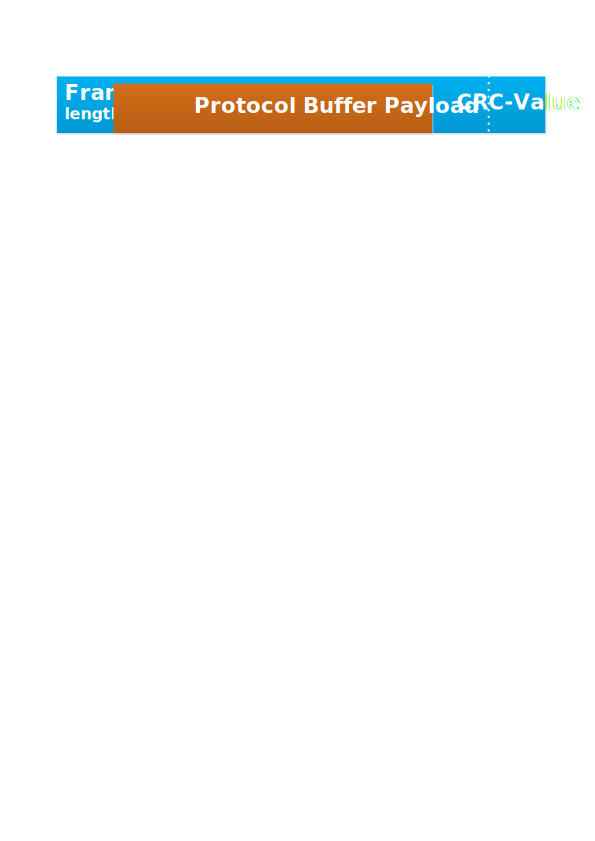
\includegraphics[width=\textwidth]{MessageFormat}
  \caption{Schematischer Aufbau eines Frames}
  \label{fig:FrameOv}
\end{figure}
\subsubsection{Sensordaten Nachricht}
Bei der Absprache mit den für die GUI verantwortlichen Entwicklern, kam folgende Anforderung hinzu: "Die Nachrichten sollen mit einem Zeitstempel oder einer fortlaufenden Nummer ausgestattet sein, um diese später unter Umständen nochmals sortieren zu können." Um auch für zukünftige Erweiterungen von Sensoren gerüstet zu sein, soll die Anzahl der Sensordaten in der Nachricht variabel gestaltet sein. Zudem wird jedem Sensorwert die ID des Sensors, welcher den Wert produzierte, zugeordnet. Um das alles zu erfüllen gilt für die Protobuf Nachricht folgende Beschreibung:
\begin{lstlisting}[caption=Beschreibung der Sensordaten Nachricht, label=lst:protoData]
//defining an entry of the data table
message DataEntry{
	uint32 SensorId = 1;
	double Data = 2;
}
//defining the real message
message SensorMsg{
	//Upcounting Nr
	uint64 SequenceNr = 1;
	//all Data
	repeated DataEntry DataTable = 2;
}
\end{lstlisting}
\subsubsection{Regelungsparameter Nachricht}
Das Team, welches die Regelung umgesetzt hat, stellt eine API bereit, welche neben den Parametern der P-, I- und D-Glieder eines Reglers auch die Regelgröße (z.B. Geschwindigkeit oder Drehmoment) und den Zielwert entgegennimmt. Dazu müssen diese Werte auch in der Protobuf Nachricht wie folgt berücksichtigt werden:
\begin{lstlisting}[caption=Beschreibung der Parameter Nachricht, label=lst:protoPara]
//defining the parameter message
message RegParams{
	uint32 target = 1;
	float paraP = 2;
	float paraI = 3;
	float paraD = 4;
	float tgtVal = 5;
}
\end{lstlisting}
Im Codebeispiel \ref{lst:protoPara} wird die Regelgröße mittels dem "target" Feld übermittelt. Dabei muss jedoch beachtet werden, dass bei beiden Kommunikationspartnern die Werte der gleichen Größe zugeordnet werden.
\subsection{Schnittstellendefinition}
\subsubsection{PC Bibliothek}
Für den Teil, welcher die Kommunikation auf Seiten der GUI übernimmt, soll eine Bibliothek auf C\#-Basis implementiert werden. Um nun Regelungsparameter an den Controller senden zu können, muss ein Datenobjekt beim Aufruf der Sende-Methode übergeben werden. Für den Empfang von Sensordaten ist es von Vorteil, das Hollywood-Prinzip anzuwenden. So soll die Bibiliothek nicht regelmäßig nach neuen Daten abgefragt werden. Vielmehr lößt deren API ein Event aus, welches die Verfügbarkeit neuer Werte anzeigt. Da sich bereits darauf festgelegt wurde, einen virtuellen Com-Port zur Kommunikation zu verwenden, soll dieser nun auch bei der Initialisierung der API als String oder gleich als ComPort-Objekt mit angegeben werden. 
\subsubsection{Controller Funktionen}
Ähnlich zur PC Bibliothek sollen die Funktionen auf dem $\mu$-Controller aufgebaut werden. Es soll zunächst eine Funktion zur Initialisierung der Kommmunikation bereitgestellt werden. Darüber hinaus soll es eine Funktion zum Setzen und eine weitere zum Versenden der gesammelten Sensordaten geben. Während der Analysephase wurde ersichtlich, dass auf dem Controller ein DMA-Baustein (Direct Memory Access) genutzt werden kann, um die Nachrichten-Bytes vom und zum UART-Modul zu übertragen. Dies erleichtert die Handhabung der Kommunikationsfunktionen dahingehend, dass nun beim erfolgreichen Empfang von Regelungsparametern ein globales Flag gesetzt werden kann, welches dies gegenüber der Regelungsschleife anzeigt. Eine weitere Aktion bezüglich des Datenempfangs von Seiten der Regelung ist somit nicht erforderlich. Die so empfangenen Regelungsparameter sollen nun nach Erhalt in global sichtbare Variablen abgelegt werden. Dies geschieht auf Wunsch des für die Regelung verantwortlichen Teams.
\section{Implementierung}
Da beide Endpunkte gänzlich unterschiedliche Eigenschaften und Ressourcen besitzen, gibt es zwei separate Softwareprojekte. Die Implementierung der Bibliothek erfolgt wie bereits erwähnt in C\# und unter Visual Studio 2013. Für die Implementierung des Kommunikationsmoduls auf dem Controller wird die Programmiersprache C unter DAVE 4 genutzt. 
\subsection{PC Bibliothek}
\begin{figure}
  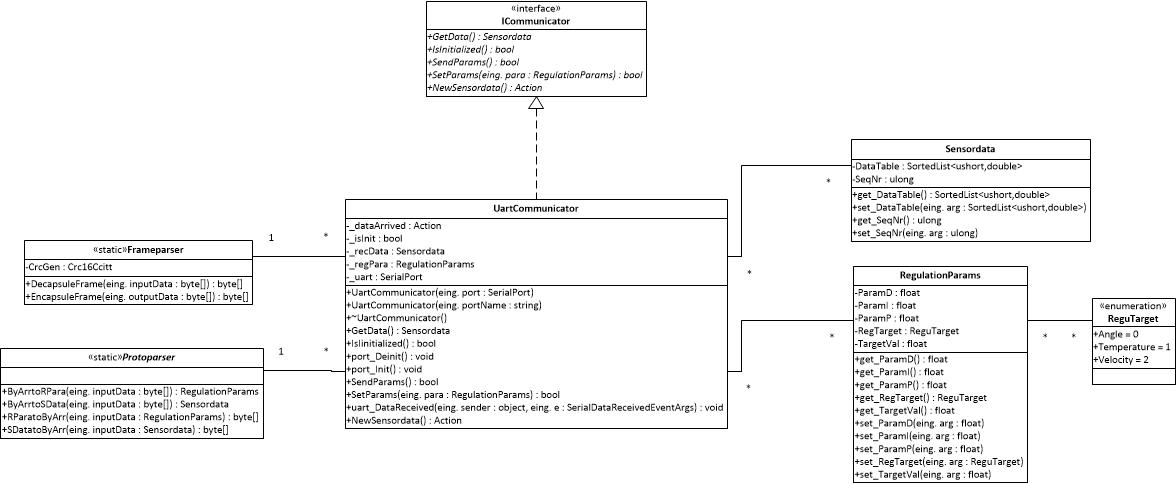
\includegraphics[width=\textwidth]{LibraryClasses}
  \caption{wesentliche Klassen der implementierten Bibliothek für die GUI}
  \label{fig:guiclasses}
\end{figure}
Wie aus Bild \ref{fig:guiclasses} ersichtlich ist, dient das Interface "ICommunicator" als API zur GUI hin und die Klasse UartCommunicator ist die Hauptklasse. Diese versammelt alle Funktionalität zum Senden und Empfangen von Nachrichten in sich. Bei der Erstellung eines Objektes dieser Klasse wird auch sofort die Initialisierungsmethode aufgerufen. In dieser wird das SerialPort-Objekt, welches zuvor dem Konstruktor angezeigt wurde, parametriert und geöffnet. Die gesetzten Parameter sind in den Zeilen 5 bis 12 im Anhang \ref{ComAPP:ComPortSettings} ersichtlich. Da zur Übertragung die USB-Schnittstelle mit nur zwei Signalleitungen genutzt wird, ist es nicht möglich für die Kommunikation einen Handshake auszuwählen bzw eine hardwaregesteuerte Flusskontrolle anzugeben. Dies wäre nur bei einer Verwendung der EIA-232 Schnittstelle möglich, da hier zusätzliche Leitungen für diese Zwecke existieren. Aus diesem Grund sind die Parameter "Handshake", "DtrEnable" und "RtsEnable" auf None bzw. false gesetzt. Alle weiteren Parameter wurden so gewählt, dass diese bereits bekannten Einstellungen für andere serielle Kommunikationen entsprechen.
\paragraph{}
Die Eigenschaft "ReceivedBytesThreshold" wurde auf 10 gesetzt. Dies bedeutet, dass nach 10 empfangenen Bytes die Methode aufgerufen wird, welche auf dem "DataReceived"-Ereignis des SerialPort-Objektes registriert wurde. Dies ist die private Methode des UartCommunicators. In dieser ist die Logik für den Empfang von Nachrichten implementiert.
\paragraph{}
Bei einem Empfang von Daten auf der seriellen Schnittstelle, wird zunächst das erste Byte im Eingangspuffer gelesen. Da dies die Framelänge darstellt (vgl. Bild \ref{fig:FrameOv}), kann nun daraus geschlossen werden, wie lang die empfangene Nachricht tatsächlich ist. Anschließend wird die nun bekannte Anzahl an Bytes in den Bearbeitungspuffer gelesen. Auf diesem Bearbeitungspuffer wird nun zunächst der Frame mit der statischen Methode "DecapsuleFrame" entpackt und folgend die Protobuf-Nachricht in ein Sensordata-Objekt umgewandelt. Am Ende der Empfangsprozedur wird das Event NewSensordata ausgelöst, welche anzeigt, dass neue Sensordaten vom UartCommunicator-Objekt abgeholt werden können. Dies geschieht mit der GetData-Methode.
\paragraph{}
Um nun Regelungsparameter versenden zu können, muss die GUI dem UartCommunicator-Objekt zunächst mit der SetParams-Methode ein Datenobjekt übergeben. Dieses Datenobjekt der Klasse RegulationParams kann nun mit der Methode "SendParams" an den Controller gesendet werden. Hier ist der Ablauf in umgekehrter Reihenfolge zu durchlaufen. Das Datenobjekt wird nun von einer statischen Methode in eine Protobuf-Nachricht serialisiert und in einen Bearbeitungspuffer abgelegt. Dieser Bearbeitungspuffer wird im Anschluss mit einem Frame-Header und einem Frame-Tail ausgestattet. Abschließend wird der Bearbeitungspuffer versendet. In Zeile 9 im Anhang \ref{ComAPP:SendWait} ist zu erkennen, dass nach jedem gesendeten Byte des Bearbeitungspuffers 30 Millisikunden gewartet wird. Dies ist notwendig, da ein kontinuierliches Senden der Datenbytes den DMA-Baustein auf dem Microcontroller überlastet und dort nur noch unverwertbare Daten vorhanden wären.
\paragraph{}
Für die Umwandlung der Daten in Protobuf-Nachrichten und umgekehrt, existiert eine separate Protoparser-Klasse. Diese stellt wie im Klassendiagramm ersichtlich statische Methoden zur Verfügung. Um aus einem Bytearray mit Protobuf-Daten ein Sensordaten-Objekt zu erzeugen, nutzt die Methode "ByArrtoSData" zunächst ein SensorMsg-Objekt aus dem durch Protobuf generierten Code. So wird ein Protobuf-Objekt erzeugt, aus welchem im Anschluss die Daten für das Sensordaten-Objekt extrahiert werden.
\paragraph{}
In die "Gegenrichtung" muss in umgekehrter Reihenfolge vorgegangen werden. Zunächst wird ein Objekt aus dem von Protobuf generierten Code mit den Daten eines Sensordata-Objektes gefüllt. Dieses Protobuf-Objekt wird nun mit der Methode "ToByteArray" in ein Array aus 8-Bit-Zahlen umgewandelt, welches wieder zurückgegeben wird. Die gleiche Vorgehensweise gilt auch für die Methoden "RParatoByArr" bzw. "ByArrtoRPara" welche die Regelungsparameter in eine Protobuf-Nachricht um- bzw. zurückwandeln.
\paragraph{}
Für die Handhabung der Nachrichten-Frames stehen in der Klasse "Frameparser" zwei statische Methoden zur Verfügung. Die Methode "DecapsuleFrame" nimmt zunächst das übergebene Byte-Array mit dem Frame und berechnet ab Element 2 die CRC-Summe. Da am Ende des Frames bereits ein 16 Bit CRC-Wert steht, entspricht das Ergebnis der aktuellen CRC-Erzeugung bei einem korrekten Frame 0. Ist dies der Fall, so werden die Bytes der Payload in einem neuen Byte-Array zurückgegeben.
\paragraph{}
Um nun ein Byte-Array mit einer Protobuf-Nachricht mit einem Frame auszustatten, existiert die statische Methode "EncapsuleFrame". Über das übergebene Array wird in dieser Methode die 16 Bit lange CRC-Summe berechnet. In ein neues Byte-Array wird nun an erster Stelle die Länge des alten Arrays + 3 als neue Framelänge abgelegt. Im Anschluss an das erste Element folgt nun das bereits übergebene Array. Abschließend werden beide Bytes des CRC-Wertes in das neue Array eingefügt, bevor dieses wieder zurückgegeben wird.
\paragraph{}
Für die Berechnung der CRC-CCITT in C\# wurde eine Klasse verwendet, welche unter sanity-free.org \cite{crc} zur Verfügung steht. Als Initialwert bei der Instanzierung wurde "NonZero1" verwendet. Es ist darauf zu achten, dass dieser Wert mit dem Initialwert auf dem $\mu$-Controller übereinstimmen muss.
\subsection{Controller Funktionen}
Die Implementierung des Kommunikationsmoduls auf dem $\mu$-Controller erfolgte unter Verwendung des Programmes DAVE 4 von Infineon. Bild \ref{fig:xmcobj}Damit ist es relativ einfach, die auf dem Chip vorhandenen Ressourcen zu parametrieren und zu nutzen. Im Rahmen der Kommunikation werden hauptsächlich zwei sogenannte Apps verwendet. Eine davon dient zur Parametrierung des UART-Bausteins, die andere zur Parametrierung der CRC-Erstellung.
\begin{figure}
  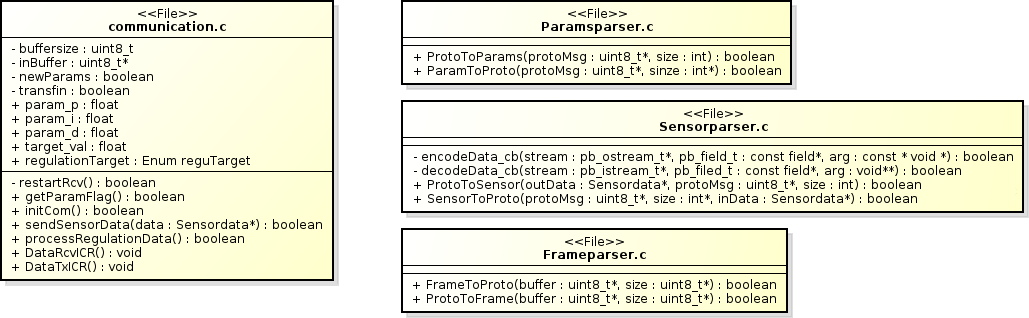
\includegraphics[width=\textwidth]{XMCObjects}
  \caption{Implementiertie Funktionen des Kommunikationsmoduls auf dem $\mu$-Controller}
  \label{fig:xmcobj}
\end{figure}
\paragraph{}
Als Hauptobjekt der API dient die Datei communication.c. Hier wird zunächst die Funktion \\"initCom" zur Verfügung gestellt. Damit werden die globalen Variablen zur Übergabe der Regelungsparameter auf einen definierten Anfangszustand gebracht und der Empfang von Nachrichten auf dem UART-Baustein angestoßen. Dazu wird die Funktion "UART\_Receive" genutzt, welche vom Programm DAVE bei Verwendung der UART-App automatisch generiert werden kann. Allerdings wird hier nur ein Byte gelesen. Denn nach der Definition des Frameaufbaus, resultiert daraus die Framelänge. Ist dieses Byte erfolgreich gelesen worden, so wird die Callback-Funktion "DataRcvICR" durch einen Interrupt aufgerufen.
\paragraph{}
In dieser Callback-Funktion wird nun ein Bearbeitungspuffer passend für den Empfangenen Frame erstellt und in diesem die noch fehlenden Bytes eines nach dem anderen abgelegt. Wurde nun der gesamte Frame erfolgreich empfangen, so wird ein Flag gesetzt. Falls nicht, wird die Kommunikation neu initialisiert.
\paragraph{}
Darüber hinaus existiert eine Funktion, welche bei ihrem Aufruf das Flag aus der Callback-Funktion zurückgibt und so anzeigt, ob eine neue Nachricht mit Regelungsparametern vorliegt. Wird hier true zurückgegeben, kann die Regelung die Funktion "processRegulationData" aufrufen. Damit wird die Verarbeitung der empfangenen Datenbytes und das erneute Empfangen von Nachrichten angestoßen.
\paragraph{}
Um nun die Daten der Sensoren zu versenden, kann die Funktion "sendSensorData" genutzt werden. Dieser muss ein Pointer auf eine Struktur des Typs "Sensordata" mit übergeben werden. Diese Funktion nun wandelt die übergebenen Daten zunächst in eine Protobuf-Nachricht und dann in einen Frame um. Dann wird dieser Frame mit der von DAVE generierten Funktion "UART\_Transmit" übertragen. Da in der Entwurfsphase beschlossen wurde, dass die Übertragung der Daten vom und zum UART-Baustein mittels DMA geschieht, gibt es für den Interrupt eines erfolgreichen Versendens der Daten eine Callback-Funktion. In dieser Funktion wird ein statisches Flag gesetzt, welches verhindert, dass der DMA-Baustein erneut Daten senden muss, obwohl die "alte" Nachricht noch nicht komplett versendet worden ist.
\paragraph{}
Für die Umwandlung der Sensordaten in eine Protobuf-Message, steht die Funktion "SensorToProto" in der Datei Sensorparser.c zur Verfügung. In dieser wird zunächst eine von nanopb generierte Struktur soweit wie möglich ausgefüllt. Um jedoch das wiederholte Feld für die sogenannte "DataTable" auszufüllen, muss eine Callback-Funktion definiert werden. Dies ist die in der gleichen Datei befindliche "encodeData\_cb". Mit dem Aufruf der ebenfalls durch nanopb generierte Funktion "pb\_encode" wird nun die Message-Struktur in ein Byte-Array umgewandelt.
\paragraph{}
In der Callback-Funktion muss für jeden Eintrag in der "DataTable" aus der Protobuf-Message die funktion "pb\_encode\_submessage" aufgerufen werden. Funktionen zum decodieren der Sensordaten-Nachricht wurden in der gleichen Datei implementiert, werden hier jedoch nicht weiter ausgeführt, da diese im Rahmen des Projektes nicht genutzt werden.
\paragraph{}
Um nun empfangene Nachrichten mit Regelungsparametern dekodieren zu können, wird die in der Datei Paramsparser.c implementierte Funktion "ProtoToParams" genutzt. Aufgrund des einfacheren Aufbaus der Parameter-Message, müssen hier nach dem Aufruf der generierten Funktion "pb\_decode" nur die Parameterwerte aus einer temporären Struktur in die zuvor genannten, globalen Variablen übertragen werden. Auch in dieser Datei existiert wieder eine Funktion, welche Regelungsparameter in eine Protobuf-Nachricht umwandelt. Auch diese wurde nur der Vollständigkeit wegen implementiert und wird im Projekt nicht genutzt.
\paragraph{}
Zum Ein- und Entpacken der Messages in Frames, können die Funktionen "ProtoToFrame" bzw. "FrameToProto" aus der Datei Frameparser.c genutzt werden. Bei der Erstellung des Frames wird der übergebene Puffer auf die richtige Größe gebracht. Weiter werden am Anfang die Anzahl der Bytes des gesamten Frames und am Ende zwei Bytes mit dem CRC-Wert abgelegt. Um diesen Wert zu erhalten werden die durch DAVE generierten Funktionen "CRC\_SW\_CalculateCRC" sowie "CRC\_SW\_GetCRCResult" genutzt. Bei der Nutzung der Funktion "ProtoToFrame" ist darauf zu achten, dass das erste Element des übergebenen Puffers keine Daten der Payload enthält, da hier die Framelänge abgelegt wird.
\paragraph{}
In der Funktion "FrameToProto" werden auch die genannten Funktionen zur Generierung des CRC-Wertes genutzt. Hier wird jedoch das Ergebnis auf 0 überprüft. Wie bereits geschildert, bedeutet beim Entkapseln des Frames ein CRC-Wert gleich 0, dass kein Fehler während der Übertragung aufgetreten ist. Ist dies der Fall, so wird der Bearbeitungspuffer um 2 Elemente verkleinert. Das dritte nun überschüssige Byte des Puffers wird nicht gelöscht, da ein dadurch notwendiges Verrücken der Payload im Puffer zu ressourcenintensiv ist. Allerdings wird die Größe der Payload durch die Funktion "FrameToProto" richtig zurückgegeben.
\paragraph{}
Außerdem existieren noch zwei Header-Dateien com\_types.h und SensorIDs.h. In der Ersteren befinden sich die Definitionen für die Sensordata-Struktur, welche die Regelung zur Übergabe der Sensorwerte nutzt, sowie der Aufzählung der möglichen Regelgröße. In der Letzteren wurden die ID's der einzelnen Sensoren für die Zuordnung der Werte abgelegt.
\subsection{Parametrierung der DAVE Apps}
In den Bildern \ref{fig:dave1} bis \ref{fig:dave6} werden alle in den DAVE Apps getroffenen Einstellungen aufgeführt. Die notwendigen Apps "UART [4.1.8]" und "CRC\_SW [4.0.6]" werden über den Menüpunkt "DAVE -> Add New APP ..." hinzugefügt.
\newpage
\begin{figure}[!h]
  \begin{minipage}{0.4\textwidth}
    \centering
    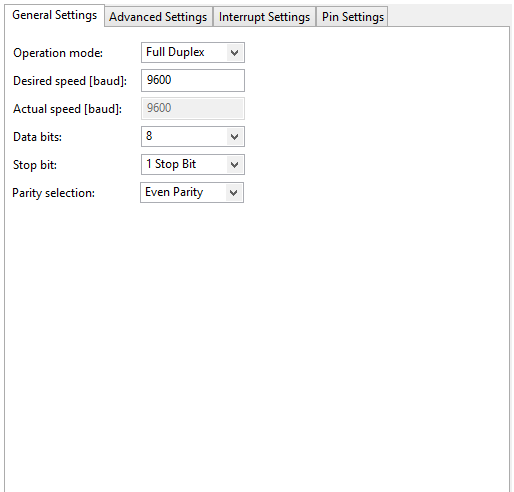
\includegraphics[width=\textwidth]{UARTgeneralSet}
    \caption{Grundlegende Einstellungen der UART-App: Diese müssen mit den Einstellungen der PC-Bibliothek übereinstimmen.}
    \label{fig:dave1}
  \end{minipage}
  \begin{minipage}{0.4\textwidth}
    \centering
    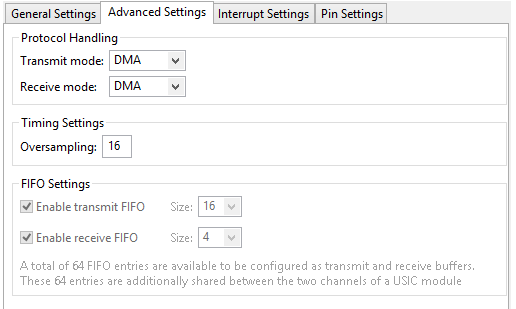
\includegraphics[width=\textwidth]{UARTadvancedSet}
    \caption{Weiterführende Einstellungen der UART-App: Beide Richtungen werden per DMA gehandhabt.}
  \end{minipage}
  \begin{minipage}{0.4\textwidth}
    \centering
    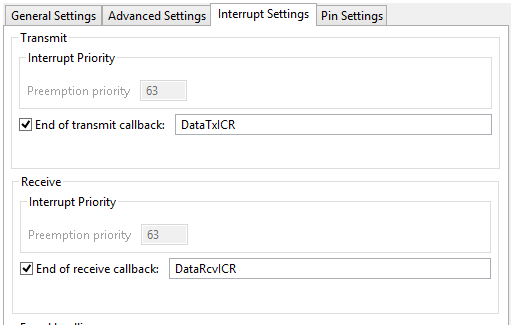
\includegraphics[width=\textwidth]{UARTinterSet}
    \caption{Interrupt Einstellungen der UART-App: Hier werden die Callback-Funktionen angegeben.}
  \end{minipage}
  \begin{minipage}{0.4\textwidth}
    \centering
    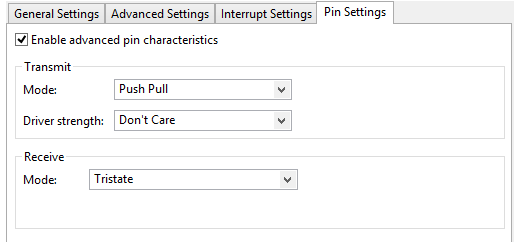
\includegraphics[width=\textwidth]{UARTpinSet}
    \caption{GPIO Einstellungen der UART-App}
  \end{minipage}
  \begin{minipage}{0.4\textwidth}
    \centering
    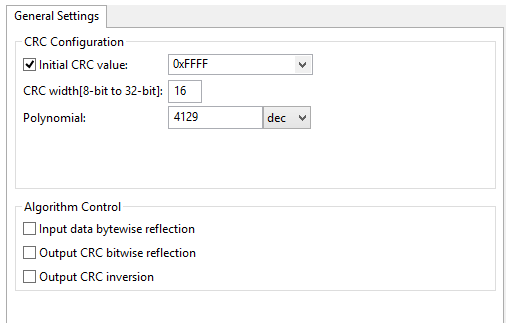
\includegraphics[width=\textwidth]{CRCgeneralSet}
    \caption{Einstellungen der CRC-App: Auch hier müssen die Einstellungen mit denen der PC-Bibliothek übereinstimmen.}
  \end{minipage}
  \begin{minipage}{0.4\textwidth}
    \centering
    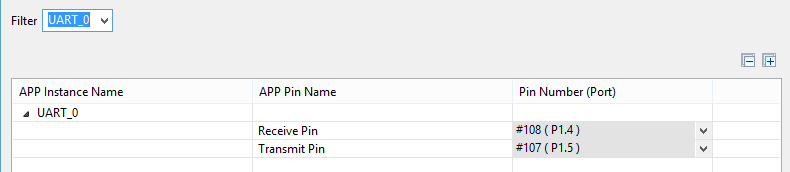
\includegraphics[width=\textwidth]{PinAlloc}
    \caption{Zuordnung der GPIO-Pins unter "DAVE -> Manual Pin Allocator"; Die Pins P1.4 und P1.5 sind mit dem Debug-Chip verbunden. Siehe \cite[Table 5]{boardMan}}
    \label{fig:dave6}
  \end{minipage}
\end{figure}
\newpage
\section{Integration}
\begin{figure}
  
\includegraphics[width=\textwidth]{WorkBufferFail}
  \caption{Inhalt eines falsch interpretierten Bearbeitungspuffers}
  \label{fig:FrameFail}
\end{figure}
Die Integration der beiden Module in die Regelung erfolgte hauptsächlich durch Herrn Krupinski. Auf Seiten der GUI übernahm diese Aufgabe Herr Krause. Herr Schleinkofer war in beiden Fällen nur beratend tätig. Seine Hauptaufgabe während dieser Phase bestand in der Behebung der auftretenden Fehler. Bei einem ersten Zusammenfügen von Regelung und GUI wurde ersichtlich, dass das Senden der Nachrichten mit den Sensorwerten nur unzureichend robust war. Die Ursache bestand hauptsächlich im Design der Nachrichten und des Kommunikationsablaufs. Sind im Eingangspuffer des SerialPort-Objekts noch Rest-Daten, so interpretiert die Kommunikationsbibliothek diese fälschlicherweise als Beginn einer neuen Nachricht. Das erste Byte wird daher als Framelänge interpretiert. Ein neuer Frame wird dann nur unvollständig in den Bearbeitungspuffer übernommen (siehe Bild \ref{fig:FrameFail}). So befindet sich dort am Anfang die Hälfte der alten Nachricht und am Ende der Anfang der neuen. Dies führt zu einem Verwerfen des Inhalts im Bearbeitungspuffer. Dieses Verhalten wiederholt sich nun im weiteren Programmverlauf, sodass nun keine Sensordaten mehr empfangen werden können. Sender und Empfänger sind nicht mehr im "gleichen Takt". 
\paragraph{}
\begin{figure}
  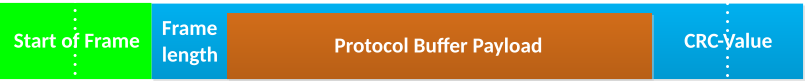
\includegraphics[width=\textwidth]{MessageFormat_enhanced}
  \caption{Verbessertes Nachrichtendesign mit Start of Frame}
  \label{fig:FrameEnhanced}
\end{figure}
Um dies zu verhindern, wird nun zu Beginn jedes Frames vom $\mu$-Controller ein 16 Bit langer Start of Frame Delimiter (kurz: SoF) mit übertragen (siehe Bild \ref{fig:FrameEnhanced}). Es ist bei der Wahl des SoF darauf zu achten, dass diese Bitreihenfolge möglichst einzigartig in der Kommunikation ist. Aus Bekanntheitsgründen und mangels Vergleichswerten aus der vorliegenden Kommunikation wurde dabei auf einen Teil des Musters eines Ethernet-Frames gewählt. Das erste Byte des SOF ist 0x55 und das zweite 0xD5. Es wären aber auch andere Werte denkbar. Die Bibliothek prüft nun vor dem Verarbeiten eines Frames, ob am Anfang des SerialPort-Eingangspuffers nun diese zwei Bytes vorhanden sind. Dies geschieht mittels eines einfach implementierten Zustandsautomaten. In einer Schleife wird nun immer das erste Byte des Eingangspuffers gelesen und verworfen. Folgendes Bild verdeutlicht den im Anhang \ref{ComAPP:SoFMachine} implementierten Automaten.
\begin{figure}
  \centering
  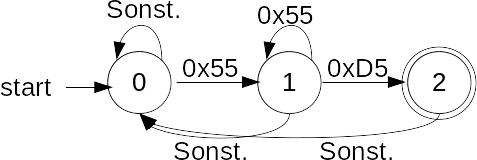
\includegraphics[width=0.4\textwidth]{Automat}
  \caption{Zustandsautomat zur erkennung des Start of Frame}
  \label{fig:Machine}
\end{figure}
\section{Ausblick}
Leider war bereits ab der Hälfte der Bearbeitungszeit absehbar, dass die anderen Arbeitspakete zeitmäßig nicht mehr auf den XE16x portiert werden können. Deshalb wurde auch das Kommunikations-Modul nicht mehr für den bisher in der Vorlesung Embedded Systems verwendeten Controller umgesetzt. Stattdessen war Herr Schleinkofer in anderen Arbeitspaketen (v.a. der Simulation) unterstützend tätig. Die Umsetzung des Projektes auf den zweiten Chip ist im Nachgang dieses Projektes noch möglich.
\paragraph{}
Einige Funktionen für eine zuverlässige Kommunikation konnten aufgrund der beschränkten Zeit ebenfalls nicht mehr umgesetzt werden. So ist es von Vorteil, wenn auch die Nachrichten mit den Regelungsparametern einen Start of Frame vorangestellt bekommen. Dies würde wie auch auf der GUI-Seite verhindern, dass eine unvollständig empfangene Nachricht das Erkennen eines Framebeginns verhindert.
\paragraph{}
Darüber hinaus wäre noch vorstellbar, für die Übertragung der Regelungsparameter eine Empfangsbestätigung zu implementieren. Dies würde einem eventuell notwendigen mehrfachen Sendeversuch durch den Benutzer vorbeugen.
\paragraph{}
Weiterhin wurde bei einem Review des erstellten Codes ersichtlich, dass die DAVE-App zur Erzeugung des CRC-Wertes keinen Gebrauch der Flexible CRC Engine auf dem $\mu$-Controller macht. Aufgrund des Zeitdrucks war eine detailliertere Einarbeitung in die Parametrierung der Hardware nicht mehr möglich.
